\documentclass[aspectratio=169,10pt]{beamer}

\usetheme[block=fill,progressbar=foot,background=light]{metropolis}   
\setbeamercolor{background canvas}{bg=white}
\usepackage{appendixnumberbeamer}

\title{Introduction au DevOps}
\subtitle{Introduction}
\date{12 Septembre 2025}
\author{Jolan PHILIPPE}
\institute{Université d'Orléans}

\usepackage{graphicx}
%\usepackage{cite}
\usepackage{subcaption}
\usepackage{lmodern}
\usepackage{hyperref}
\usepackage{array}
\usepackage{multirow}
%\usepackage[table]{xcolor}
\usepackage{mathabx}
\usepackage{amsmath}
\usepackage{amssymb}
\usepackage{wrapfig}
\usepackage{fancyhdr}
\usepackage{url}
\usepackage{listings}
\usepackage{minted}
\usepackage{fontawesome}
\usepackage{tikz}
\usepackage{hyperref}
\usetikzlibrary{automata, positioning, matrix, fit}
\usetikzlibrary{arrows.meta,calc,decorations.markings,math}
\usetikzlibrary{shadows.blur}
\usetikzlibrary{decorations.pathreplacing, fit}
\usetikzlibrary{shapes,arrows}
\usepackage{flushend}
\usepackage{ifthen}
\newboolean{showtodos}

% ----------------------------------------
% COLORS
\definecolor{gray}{rgb}{0.5,0.5,0.5}
\definecolor{ashgrey}{rgb}{0.7, 0.75, 0.71}
\definecolor{battleshipgrey}{rgb}{0.52, 0.52, 0.51}
\definecolor{aliceblue}{rgb}{0.94, 0.97, 1.0}
\definecolor{mauve}{rgb}{0.58,0,0.82}
\definecolor{auburn}{rgb}{0.43, 0.21, 0.1}
\definecolor{babyblue}{rgb}{0.54, 0.81, 0.94}
\definecolor{amaranth}{rgb}{0.9, 0.17, 0.31}
\definecolor{bleudefrance}{rgb}{0.19, 0.55, 0.93}
\definecolor{atomictangerine}{rgb}{1.0, 0.6, 0.4}
\definecolor{beaublue}{rgb}{0.74, 0.83, 0.9}
\definecolor{dkviolet}{rgb}{0.9, 0.17, 0.31}
\definecolor{dkgreen}{rgb}{0.0, 0.42, 0.24}
\definecolor{ltblue}{rgb}{0.0, 0.75, 1.0}
\definecolor{dkblue}{rgb}{0.2, 0.2, 0.6}
\definecolor{dkred}{rgb}{0.8, 0.0, 0.0}
\definecolor{byzantine}{rgb}{0.74, 0.2, 0.64}
% ----------------------------------------



\usepackage[textwidth=17mm]{todonotes}
\newcommand{\instructions}[1]{
	\todo[color=black!20,inline,size=\small]{#1}
}
\newcommand{\customtodo}[4]{
\ifthenelse{\boolean{showtodos}} { 
	\todo[color=#2,inline,size=\small]{
		\ifx&#3&
		\textbf{#1} #4
		\else
		\textbf{#1$\Rightarrow$#3} #4
		\fi
	}
 } 
}{}

\newcommand{\jolan}[2][]{\customtodo{Jolan}{pink!40}{#1}{#2}}
\newcommand{\antoine}[2][]{\customtodo{Antoine}{red!40}{#1}{#2}}
\newcommand{\helene}[2][]{\customtodo{Helene}{orange!40}{#1}{#2}}
\newcommand{\issam}[2][]{\customtodo{Issam}{green!40}{#1}{#2}}
\newcommand{\charles}[2][]{\customtodo{Charles}{blue!40}{#1}{#2}}

\newcommand{\tmp}[1][]{\customtodo{To remove}{gray}{#1}}

\usepackage{xspace}
\newcommand{\ie}[0]{{\em i.e.},\xspace}
\newcommand{\vs}[0]{{\em vs.}\xspace}
\newcommand{\eg}[0]{{\em e.g.},\xspace}
\newcommand{\etal}[0]{{\em et al.}\xspace}
\newcommand{\wrt}[0]{{\em w.r.t.}\xspace}
\newcommand{\aka}[0]{{\em a.k.a.}\xspace}
\newcommand{\via}[0]{{\em via}\xspace}

% ----------------------------------------

\lstdefinestyle{goalstyle}{
  basicstyle=\scriptsize\itshape,
  xleftmargin=1em,
  literate={::=}{$::=$}{2},
  keywords={behaviors,ports,components,forall,component,behavior,port,status}
}

\lstdefinelanguage{MiniZinc}{
numberstyle=\tiny\color{gray},
% Anything betweeen $ becomes LaTeX math mode
mathescape=true,
% Comments may or not include Latex commands
texcl=false,
% Vernacular commands
morekeywords=[1]{ann, annotation, any, array, assert,
        bool,
        constraint,
        else, elseif, endif, enum, exists,
        float, forall, function,
        if, in, include, int,
        list,
        minimize, maximize,
        of, op, output,
        par, predicate,
        record,
        set, solve, string,
        test, then, tuple, type,
        var,
        where,
        %% MiniZinc functions
        %%
        abort, abs, acosh, array_intersect, array_union,
        array1d, array2d, array3d, array4d, array5d, array6d, asin, assert, atan,
        bool2int,
        card, ceil, combinator, concat, cos, cosh,
        dom, dom_array, dom_size, dominance,
        exp,
        fix, floor,
        index_set, index_set_1of2, index_set_2of2, index_set_1of3, index_set_2of3, index_set_3of3,
        int2float, is_fixed,Yaml
        join,
        lb, lb_array, length, let, ln, log, log2, log10,
        min, max,
        pow, product,
        round,
        set2array, show, show_int, show_float, sin, sinh, sqrt, sum,
        tan, tanh, trace,
        ub, and ub_array,
        %% Search keywords
        bool_search, int_search, seq_search, priority_search,
        %% MiniSearch keywords
        minisearch, search, while, repeat, next, commit, print, post, sol, scope, time_limit, break, fail},
numbers=left,
% Gallina
morekeywords=[2]{Array},
% Spaces are not displayed as a special character
showstringspaces=false,
% String delimiters
morestring=[b]",
morestring=[d]',
% Size of tabulations
tabsize=2,
% Enables ASCII chars 128 to 255
extendedchars=false,
% Case sensitivity
sensitive=true,
% Automatic breaking of long lines
breaklines=false,
% Default style fors listings
basicstyle=\footnotesize,
% Position of captions is bottom
captionpos=b,
% flexible columns
basewidth={2em, 0.5em},
columns=[l]flexible,
% Style for (listings') identifiers
identifierstyle={\ttfamily\color{black}},
% Style for declaration keywords
keywordstyle=[1]{\ttfamily\bfseries\color{dkviolet}},
% Style for gallina keywords
keywordstyle=[2]{\ttfamily\bfseries\color{dkgreen}},
% Style for strings
stringstyle=\ttfamily,
% Style for comments
commentstyle={\ttfamily\itshape\color{dkgreen}},
%moredelim=**[is][\ttfamily\color{red}]{/&}{&/},
literate=
  {forall}{{\color{dkgreen}{$\forall$}}}1
{exists}{{$\exists$}}1
{<-}{{$\leftarrow$}}1
{=>}{{$\Rightarrow$}}1
%{==}{{\code{==}}}1
%{==>}{{\code{==>}}}1
%    {:>}{{\code{:>}}}1
{->}{{$\rightarrow$}}1
{<-->}{{$\longleftrightarrow$}}1
{<->}{{$\leftrightarrow$}}1
{<==}{{$\leq$}}1
{\#}{{$^\star$}}1
{\\o}{{$\circ$}}1
%    {\@}{{$\cdot$}}1 
{\/\\}{{$\wedge$}}1
{\\\/}{{$\vee$}}1
%{++}{{\code{++}}}1
{~}{{\ }}1
{\@\@}{{$@$}}1
{\\mapsto}{{$\mapsto$}}1
{\\hline}{{\rule{\linewidth}{0.5pt}}}1
%
}[keywords,comments,strings]
\lstdefinestyle{mznstyle}{
  language=MiniZinc,
}
% ----------------------------------------
\lstdefinelanguage{MyPython}{
morekeywords=[1]{def, if, while, return, not},
morekeywords=[5]{get_messages, infer_constraints, plan_inference, infer_messages, bhv_inference, send_messages, allAcked, send_ack, ack, global_ack},
keywordstyle=[5]{\ttfamily\bfseries\color{purple}},
tabsize=2,
numbers=left,
numberstyle=\tiny\color{gray},
breaklines=true,
basicstyle=\footnotesize,
% literate= 
% {act_c}{{$act_c$}}1
% {Gbhv}{{$\Gamma bhv$}}1
% {Gfinal}{{$\Gamma final$}}1,
% {Gbhv_c}{{$\Gamma bhv_{c}$}}1
% {Gport_c}{{$\Gamma port_{c}$}}1
% {Gfinal_c}{{$\Gamma final_{c}$}}1
}
\lstdefinestyle{pythonstyle}{language=MyPython}
\lstMakeShortInline[language=MyPython]"

\newfloat{Model}{t}{lom}
\newcommand{\constraint}[1]{\textnormal{\textsc{#1}}}
\newcommand{\Regular}{\constraint{Regular}}
\newcommand{\CostRegular}{\constraint{CostRegular}}
\newcommand{\Count}{\constraint{Count}}
\newcommand{\Element}{\constraint{Element}}
\newcommand{\Sum}{\constraint{Sum}}

%------------------------------------------------------
\definecolor{codegreen}{rgb}{0,0.6,0}
\definecolor{codegray}{rgb}{0.5,0.5,0.5}
\definecolor{codepurple}{rgb}{0.58,0,0.82}
\definecolor{backcolour}{rgb}{0.95,0.95,0.92}
\lstdefinestyle{mystyle}{
    commentstyle=\color{codegreen},
    keywordstyle=\color{purple},
    tabsize=2,
    numbers=left,
    numberstyle=\tiny\color{gray},
    stringstyle=\color{codepurple},
    breaklines=true,
    basicstyle=\tiny
}


\definecolor{keywords}{RGB}{255,0,90}
\definecolor{comments}{RGB}{0,0,113}
\definecolor{red}{RGB}{160,0,0}
\definecolor{green}{RGB}{0,150,0}
\definecolor{backcolour}{rgb}{0.95,0.95,0.95}
\DeclareCaptionFont{white}{\color{white}}
\DeclareCaptionFont{gray}{\color{gray}}
\DeclareCaptionFormat{listing}{\colorbox{backcolour}{\parbox{\linewidth}{#1#2#3}}}
\captionsetup[lstlisting]{format=listing}%,labelfont=white,textfont=white}
\lstdefinestyle{mystyle}{
    tabsize=2,
    numberstyle=\tiny\color{gray},
    breaklines=true,
    numbers=left,
    backgroundcolor=\color{white},
    numbersep=5pt,
    keywordstyle=\color{keywords},
    commentstyle=\color{comments},
    stringstyle=\color{blue},
    showstringspaces=false,
    identifierstyle=\color{green},
    basicstyle=\scriptsize\ttfamily,
    numberstyle=\tiny\color{gray},
}

\lstdefinestyle{mysmallstyle}{
    tabsize=2,
    numberstyle=\tiny\color{gray},
    breaklines=true,
    numbers=left,
    backgroundcolor=\color{white},
    numbersep=5pt,
    keywordstyle=\color{keywords},
    commentstyle=\color{comments},
    stringstyle=\color{blue},
    showstringspaces=false,
    identifierstyle=\color{green},
    basicstyle=\scriptsize\ttfamily,
    numberstyle=\tiny\color{gray},
}

\lstdefinestyle{yaml}{
     basicstyle=\color{black}\scriptsize,
     keywords =[1]{behaviors, components, connections},
    keywordstyle=[1]{\color{blue}\scriptsize}, 
     rulecolor=\color{black},
     string=[s]{'}{'},
     stringstyle=\color{blue},
     comment=[l]{:},
     commentstyle=\color{black},
     morecomment=[l]{-}
 }

\usepackage{pifont,utfsym}
\newcommand{\cmark}{\ding{51}}
\newcommand{\xmark}{\ding{55}}
\newcommand{\OKmark}{{\color{green}\cmark}}
\newcommand{\KOmark}{{\color{red}\xmark}}



% \usetikzlibrary{positioning, arrows.meta, decorations.pathreplacing, fit}
% \pgfarrowsdeclare{lollipop}{lollipop}{
%     \pgfsetlinewidth{0.7pt}
%     \pgfarrowsleftextend{0pt}
%     \pgfarrowsrightextend{2pt}
% }{
%     \pgfpathcircle{\pgfpoint{0pt}{0pt}}{2pt}
%     \pgfusepathqfillstroke
% }
% \pgfarrowsdeclare{socket}{socket}{
%     \pgfarrowsleftextend{2pt}
%     \pgfarrowsrightextend{2pt}
% }{
%     \pgfsetlinewidth{0.7pt}
%     \pgfpathmoveto{\pgfqpoint{3pt}{-3pt}}
%     \pgfpatharc{270}{90}{3pt}
%     \pgfusepathqstroke
% }

% % Define styles for lollipop and socket arrows
% \tikzset{
%   lollipop/.style={
%     -{lollipop}
%   },
%   socket/.style={
%     -{socket}
%   }
% }





% Define a new arrow tip for the lollipop (filled circle)
\pgfarrowsdeclare{lollipop}{lollipop}{
    \pgfsetlinewidth{0.7pt}
    \pgfarrowsleftextend{0pt}
    \pgfarrowsrightextend{2pt}
}{
    \pgfpathcircle{\pgfpoint{0pt}{0pt}}{2pt}
    \pgfusepathqfillstroke
}

% Define a new arrow tip for the socket (reversed C)
\pgfarrowsdeclare{socket}{socket}{
    \pgfarrowsleftextend{2pt}
    \pgfarrowsrightextend{2pt}
}{
    \pgfsetlinewidth{0.7pt}
    \pgfpathmoveto{\pgfqpoint{3pt}{-3pt}}
    \pgfpatharc{270}{90}{3pt}
    \pgfusepathqstroke
}

% Define styles for lollipop and socket arrows
\tikzset{
  lollipop/.style={
    -{lollipop}
  },
  socket/.style={
    -{socket}
  }
}

\newcommand{\simpleprovideuse}[3][1cm]{%
    \path (#2) -- (#3) coordinate[pos=0.5] (mid#2#3);
    \draw[-{lollipop}] (#2) -- (mid#2#3);
    \draw[-{socket}] (#3) -- (mid#2#3);
}

\newcommand{\provideuse}[3][1cm]{
    % Usage :
    %   \provideuse{src}{target}
    % Example:
    %   \node[draw, circle] (A) {A};
    %   \node[draw, circle] (B) {B};
    %   \provideuse{A}{B}
    \path (#2) -- (#3) coordinate[pos=0.5] (mid#2#3);
    \path (#2) -- (mid#2#3) coordinate[pos=0.5] (q1#2#3);
    \path (mid#2#3) -- (#3) coordinate[pos=0.5] (q3#2#3);
    \draw[-{lollipop}] (#2) -- (q1#2#3);
    \draw[-{lollipop}] (mid#2#3) -- (q3#2#3);
    \draw[-{socket}] (#3) -- (q3#2#3);
    \draw[-{socket}] (q3#2#3) -- (q1#2#3);
}

\newcommand{\provideusetwolabels}[5][1cm]{%
    % Usage :
    %   \provideusetwolabels{src}{target}
    % Example:
    %   \node[draw, circle] (A) {A};
    %   \node[draw, circle] (B) {B};
    %   \provideusetwolabels{A}{B}{provide}{use}
    \path (#2) -- (#3) coordinate[pos=0.5] (mid#2#3);
    \path (#2) -- (mid#2#3) coordinate[pos=0.5] (q1#2#3);
    \path (mid#2#3) -- (#3) coordinate[pos=0.5] (q3#2#3);
    \draw[-{lollipop}] (#2) --  node[midway, above, xshift=0.08cm] {\tiny #4} (q1#2#3);
    \draw[-{lollipop}] (mid#2#3) -- (q3#2#3);
    \draw[-{socket}] (#3) -- node[midway, below, xshift=-0.4cm] { \tiny #5} (q3#2#3);
    \draw[-{socket}] (q3#2#3) -- (q1#2#3);
}

\newcommand{\provideusesinglelabel}[4][1cm]{%
    % Usage :
    %   \provideusesinglelabel{src}{target}
    % Example:
    %   \node[draw, circle] (A) {A};
    %   \node[draw, circle] (B) {B};
    %   \provideusesinglelabel{A}{B}{relation}
    \path (#2) -- (#3) coordinate[pos=0.5] (mid#2#3);
    \path (#2) -- (mid#2#3) coordinate[pos=0.5] (q1#2#3);
    \path (mid#2#3) -- (#3) coordinate[pos=0.5] (q3#2#3);
    \draw[-{lollipop}] (#2) -- (q1#2#3);
    \draw[-{lollipop}] (mid#2#3) -- (q3#2#3);
    \draw[-{socket}] (#3) -- (q3#2#3);
    \draw[-{socket}] (q3#2#3)  -- node[midway, above] {\scriptsize #4} (q1#2#3);
}

\usepackage{pifont,utfsym}
\newcommand{\cmark}{\ding{51}}
\newcommand{\xmark}{\ding{55}}
\newcommand{\okmark}{\textbf{\color{green}\faCheck}}
\newcommand{\komark}{\textbf{\color{red}\faTimes}}
\newcommand{\midmark}{\textbf{\color{orange}$\sim$}}
\renewcommand{\OKmark}{\okmark~}
\newcommand{\OKOKmark}{\okmark\okmark~}
\renewcommand{\KOmark}{\komark~}
\newcommand{\MIDmark}{\midmark~}

\begin{document}

\begin{frame}
    \titlepage 
\end{frame}

% ----------------------------------------------------------------------------------

\begin{frame}{Hello world}
    
\begin{columns}[T]
\begin{column}{.3\textwidth} 
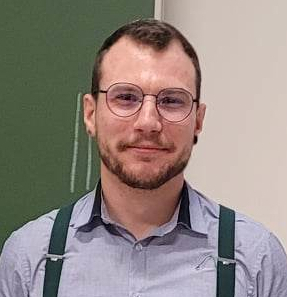
\includegraphics[scale=1]{images/jolan.jpg}
\end{column}
\hspace{-1in}
\begin{column}{.7\textwidth}

{\color{white}a}

% {\color{white}a}

Jolan Philippe, Maitre de conférence

Université d'Orléans, équipe LMV

Bureau tbd.

($\lambda$x.$\lambda$y.x@y) jolan.philippe1 univ-orleans.fr

\vspace{1cm}

\end{column}
\end{columns}

Travaux de recherche: vérification formelle de
\vspace{-0.1cm}
\begin{itemize}
    \item Programmes parallèles distribués
    \item Transformation de modèles dans les SI
    \item Déploiement d'infrastructure
\end{itemize}
Plus de détails sur  
\url{https://jolanphilippe.github.io/}
 
\end{frame}
% \maketitle

% ----------------------------------------------------------------------------------

\begin{frame}{Ce qu'on va aborder dans ce cours}

\begin{alertblock}{La philosophie DevOps}
    \begin{itemize}
        \item C'est quoi Dev ? C'est quoi Ops ?
        \item C'est quoi DevOps ?
        \item Un context particulier : le Cloud
    \end{itemize}
\end{alertblock}

\begin{alertblock}{Infrastructure-as-code}
    \begin{itemize}
        \item Conteneurisation avec Docker
        \item Provisionnement avec Terraform
        \item Configuration et gestion avec Ansible
        \item Orchestration avec Kubernetes
    \end{itemize}
\end{alertblock}
 
\end{frame}

% ----------------------------------------------------------------------------------

\section{DevOps késako ?}

% ----------------------------------------------------------------------------------

\begin{frame}{Cycle de développement}

\begin{figure}
    \centering
    \begin{tikzpicture}[
    flow/.style={
      -{Stealth[length=3mm,width=2.2mm]},
      line width=1.2pt,
      draw=black, double=white, double distance=1.1pt
    }
]


  % Boîtes
  \node[draw, rectangle, rounded corners=5, minimum height=0.8cm, minimum width=3cm] (n1) {\large Besoins};
  \node[draw, rectangle, rounded corners=5, below=0.5cm of n1, xshift=2cm, minimum height=0.8cm, minimum width=3cm] (n2) {\large Conception};
  \node[draw, rectangle, rounded corners=5, below=0.5cm of n2, xshift=2cm, minimum height=0.8cm, minimum width=3cm] (n3) {\large Execution};
  \node[draw, rectangle, rounded corners=5, below=0.5cm of n3, xshift=2cm, minimum height=0.8cm, minimum width=3cm] (n4) {\large Verification};
  \node[draw, rectangle, rounded corners=5, below=0.5cm of n4, xshift=2cm, minimum height=0.8cm, minimum width=3cm] (n5) {\large Maintenance};

  % Flèches courbes (style “double trait” + pointe)
  \draw[flow] (n1.east) to[out=-45,in=135] (n2.west);
  \draw[flow] (n2.east) to[out=-45,in=135] (n3.west);
  \draw[flow] (n3.east) to[out=-45,in=135] (n4.west);
  \draw[flow] (n4.east) to[out=-45,in=135] (n5.west);

  % (optionnel) Légende sous la figure
  % \node[below right=10pt and -15pt of n6.south east, anchor=base east]
  %   {\footnotesize \textit{Mod\`ele du cycle en cascade}};
\end{tikzpicture}

    \caption{Développement logiciel agile}
\end{figure}
 
\end{frame}

% ----------------------------------------------------------------------------------

\begin{frame}

\centering {\Huge
\textbf{Personne} ne code sans bug} 
\\
{\large(surtout avec des modifications de code régulières)}

\end{frame}

% ----------------------------------------------------------------------------------

\begin{frame}{Des bugs, c'est une certitude}

\begin{alertblock}{Windows 10 - Update causant la suppression de fichier}
    \begin{itemize}
        \item \textbf{Problème}: patch effaçant des fichiers utilisateurs lors de redirections de dossiers
        \item \textbf{Prévention}:
            \begin{itemize}
                \item Automatiser les tests, notamment en mockant la migration
                \item Déploiement progressif avec surveillance d'état du système
            \end{itemize}
    \end{itemize}
\end{alertblock}

\end{frame}

% ----------------------------------------------------------------------------------

\begin{frame}{Des bugs, c'est une certitude}

\begin{alertblock}{Firefox - Expiration d'un certificat désactivant les extensions}
    \begin{itemize}
        \item \textbf{Problème}: expiration d’un certificat de signature d’extensions
        \item \textbf{Prévention}:
            \begin{itemize}
                \item Automatiser des tests réguliers avec utilisation d'une horloge
                \item Surveillance automatisé des dates d'expirations avec des patchs automatiques
            \end{itemize}
    \end{itemize}
\end{alertblock}

\end{frame}

% ----------------------------------------------------------------------------------

\begin{frame}{Intégration continue et tests automatisés}
\begin{columns}[T,onlytextwidth]
    \begin{column}{.58\linewidth}
      \begin{alertblock}{Qu’est-ce que la CI ?}
        \begin{itemize}
          \item Fusionner le code \textbf{très fréquemment} (plusieurs fois/jour).
          \item Chaque commit déclenche \textbf{build + tests automatiques}.
          \item But : \textbf{détecter tôt} les erreurs et stabiliser le produit.
        \end{itemize}
      \end{alertblock}

    \end{column}

    \begin{column}{.38\linewidth}
      \centering
      % Schéma pipeline CI (simple)
      \begin{tikzpicture}[node distance=6mm,>=stealth,thick]
        \tikzstyle{step}=[rectangle,rounded corners,draw,align=center,minimum width=2.6cm,minimum height=0.9cm]
        \node[step] (code) {Commit\\Code};
        \node[step,below=of code] (build) {Build};
        \node[step,below=of build] (tests) {Tests\\(unit., int., lint)};
        \node[step,below=of tests,fill=green!20] (ok) {OK = Merge};
        \draw[->] (code) -- (build);
        \draw[->] (build) -- (tests);
        \draw[->] (tests) -- node[right]{\scriptsize pass} (ok);
        \draw[->,red] (tests.east) .. controls +(1,0.6) and +(1,-0.6) .. node[right]{\scriptsize fail} (code.east);
      \end{tikzpicture}
      \vspace{1ex}

      \small \emph{Prépare la suite : tests au déploiement.}
    \end{column}
  \end{columns}
 
\end{frame}

% ----------------------------------------------------------------------------------

\begin{frame}{Intégration continue et tests automatisés}

      \begin{alertblock}{Pourquoi automatiser les tests ?}
        \begin{itemize}
          \item \textbf{Réduire les régressions} liées aux patchs/maintenance.
          \item \textbf{Accélérer le feedback} aux développeurs.
          \item \textbf{Standardiser la qualité} (critères objectifs dans la pipeline).
          \item \textbf{Déployer plus souvent} avec confiance (vers CI/CD).
        \end{itemize}
      \end{alertblock}

      % \begin{alertblock}{Message clé}
      %   La CI n’apporte sa valeur que si les \textbf{tests sont automatisés} :
      %   unitaires, intégration, sécurité, performance.
      % \end{alertblock}
\end{frame}

% ----------------------------------------------------------------------------------
\begin{frame}{Tester au déploiement avec Jenkins}
  \begin{columns}[T,onlytextwidth]
    \begin{column}{.58\linewidth}
      \begin{alertblock}{Jenkins}
        \begin{itemize}
          \item \textbf{But :} valider automatiquement chaque changement de code
          \item \textbf{Déclencheurs :} webhooks Git (push/PR)
          \item \textbf{Boucle de feedback :} rapide, standardisée, versionnée.
        \end{itemize}
      \end{alertblock}

      \begin{alertblock}{Automatiser la CI}
        \begin{itemize}    
          \item \textbf{Build} reproductible 
          \item \textbf{Tests} automatisés (unitaires, intégration, lint, ...)
          \item \textbf{Qualité} : seuils (tests, couverture, lint)
          \item \textbf{Artefacts} : packaging, signature, dépôt binaire
          \item \textbf{Rapports} : notifications (chat/mail)
        \end{itemize}
      \end{alertblock}
    \end{column}

    \begin{column}{.38\linewidth}
      \centering
      \begin{tikzpicture}[node distance=5mm,>=stealth,thick]
    \node[rectangle,rounded corners,draw,align=center,
                      minimum width=2.6cm,minimum height=0.6cm,fill=blue!15] (commit) {Commit Code};
    \node[rectangle,rounded corners,draw,align=center,
                      minimum width=2.6cm,minimum height=0.6cm,fill=blue!15,below=of commit] (build) {Build};
    \node[rectangle,rounded corners,draw,align=center,
                      minimum width=2.6cm,minimum height=0.6cm,fill=blue!15,below=of build] (tests) {Tests};
    \node[rectangle,rounded corners,draw,align=center,
                      minimum width=2.6cm,minimum height=0.6cm,fill=blue!15,below=of tests] (artefact) {Artefact};
    \node[rectangle,rounded corners,draw,align=center,
                      minimum width=2.6cm,minimum height=0.6cm,fill=blue!15,below=of artefact,fill=green!20] (deploy) {Déploiement};
    \node[rectangle,rounded corners,draw,align=center,
                      minimum width=2.6cm,minimum height=0.6cm,fill=blue!15,below=of deploy,fill=orange!20] (monitor) {Monitoring};

    \node[right=0.8cm of tests]{
\includegraphics[height=2cm]{images/Jenkins.png}};
    
    \draw[->] (commit) -- (build);
    \draw[->] (build) -- (tests);
    \draw[->] (tests) -- (artefact);
    \draw[->] (artefact) -- (deploy);
    \draw[->] (deploy) -- (monitor);
\end{tikzpicture}


      \vspace{1ex}
      \small \emph{Jenkins orchestre chaque étape du pipeline.}
    \end{column}
  \end{columns}
\end{frame}

\begin{frame}
\vspace{-0.8cm}
\begin{figure}
    % \centering
    \hspace*{-1cm}% décalage vers la gauche
    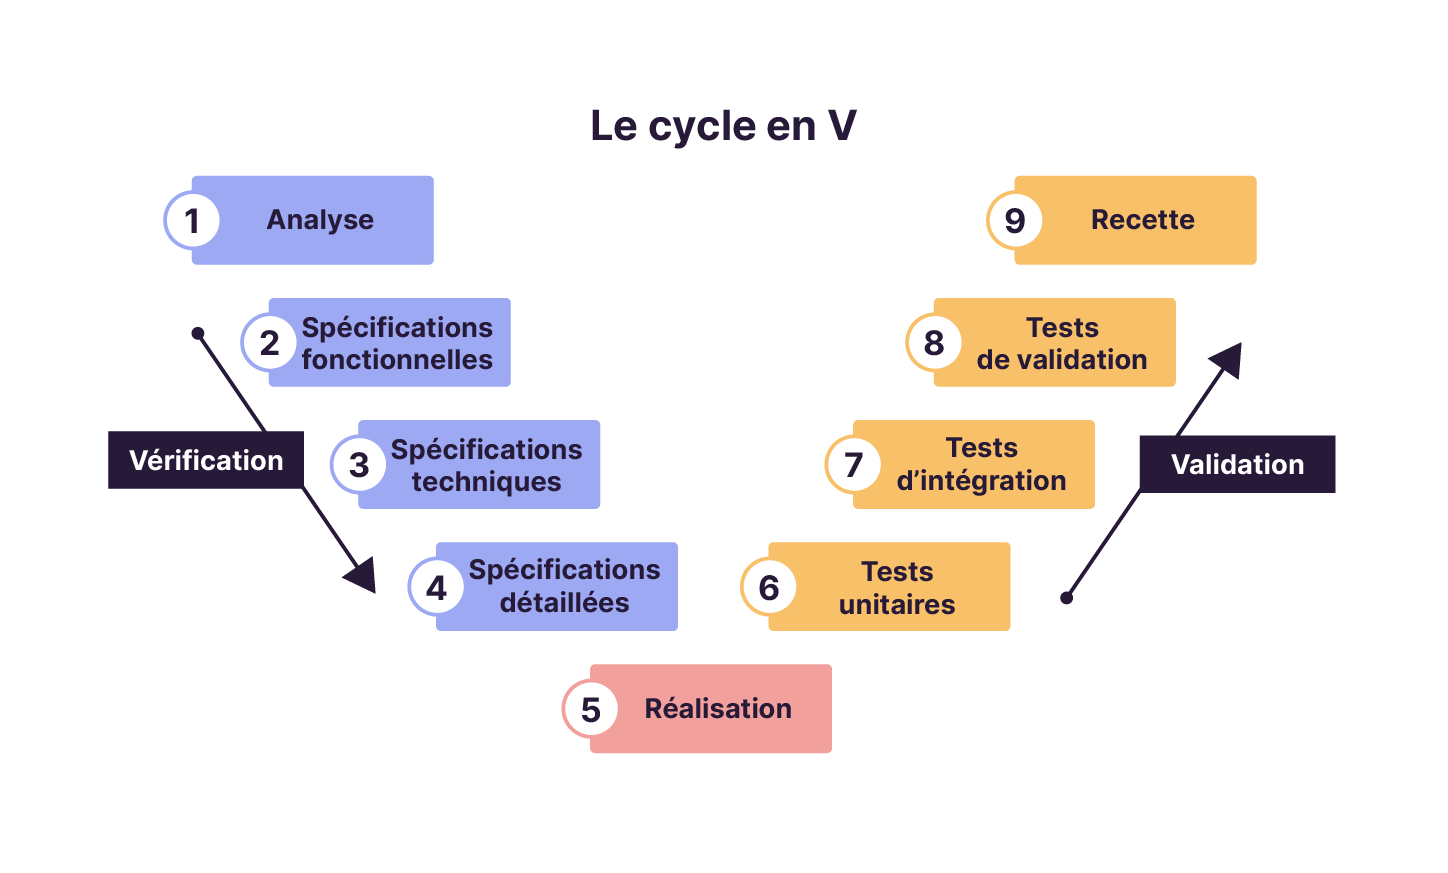
\includegraphics[scale=0.68]{figures/cycleV.png}
    \caption{Piloter un projet avec un cycle en V}
\end{figure}
 
\end{frame}

% ----------------------------------------------------------------------------------

\begin{frame}{(Vérification formelle de programmes)}

\begin{center}
    

\begin{tikzpicture}

  \node[draw, rectangle, minimum width=3cm] (n1) {
  \begin{tabular}{c}
    \large Certification;  \\
    \large Sémantique \\
    \large formelle; etc.
  \end{tabular} 
  };
  
  \node[draw, rectangle, rounded corners=15,  minimum width=3cm, right=3cm of n1] (n2) {
  \begin{tabular}{c}
    \large Programme  \\
    \large exécutable
  \end{tabular} 
  };
  
  \node[draw, rectangle, rounded corners=15,  minimum width=3cm, below=1.5cm of n1] (n3) {
  \begin{tabular}{c}
    \large Programme  \\
    \large exécutable
  \end{tabular} 
  };
  
  \node[draw, rectangle, minimum width=3cm, right=3cm of n3] (n4) {
  \begin{tabular}{c}
    \large Sémantique \\
    \large formelle
  \end{tabular} 
  };

\draw[-{Stealth[scale=2.0]}] (n1) -- node (f1) [above] {\begin{tabular}{c}
    \large Extraction \\
    \large certifiée
  \end{tabular}} (n2);

\draw[{Stealth[scale=2.0]}-{Stealth[scale=2.0]}] (n3) -- node (f2) [above] {\begin{tabular}{c}
    \large Équivalence
  \end{tabular}} (n4);

\node[above=0cm of f1] (L1) {\Large\bf Correction par construction};
\node[above=0cm of f2] (L2) {\Large\bf Correction à posteriori};

\node[below=1cm of f2] (dijsktra) {
  \begin{tabular}{c}
    \large {\it Program testing can be used to show the presence of bugs,} \\
    \large {\it but never to show their absence.} - {\bf E. W. Dijkstra }
  \end{tabular}
  };

\end{tikzpicture}
\end{center}
 
\end{frame}

% ----------------------------------------------------------------------------------

\begin{frame}{Le rôle de l'Ops}

 \begin{alertblock}{Qu’est-ce que \textbf{Ops} ?}
    \begin{itemize}
      \item La partie \textbf{Operations} du cycle DevOps.
      \item Responsable de la \textbf{mise en production}, du \textbf{monitoring}, de la \textbf{sécurité}.
      \item Objectif : \textbf{assurer la disponibilité et la fiabilité} du service.
    \end{itemize}
  \end{alertblock}

  \begin{alertblock}{Missions clés}
    \begin{itemize}
      \item Déploiement et exploitation des applications.
      \item Supervision, alertes, gestion des incidents.
      \item Automatisation des tâches d’infra (Infra as Code, scripts).
    \end{itemize}
  \end{alertblock}

\end{frame}

% ----------------------------------------------------------------------------------

\begin{frame}{Déploiement continu}

  \begin{alertblock}{Pourquoi automatiser le déploiement ?}
    \begin{itemize}
      \item \textbf{Réduire les erreurs humaines} liées aux procédures manuelles.
      \item \textbf{Déployer rapidement et fréquemment} en production.
      \item \textbf{Uniformiser} les environnements.
      \item \textbf{Sécuriser les mises en production} avec rollback rapide.
    \end{itemize}
  \end{alertblock}

Le CD rend le déploiement \textbf{fiable, répétable et rapide}, 
en s’appuyant sur l’automatisation et l’intégration avec la CI.

\end{frame}

% ----------------------------------------------------------------------------------

\begin{frame}{Mission du DevOps : Intégration continue et déploiement continu (CI/CD)}
\centering
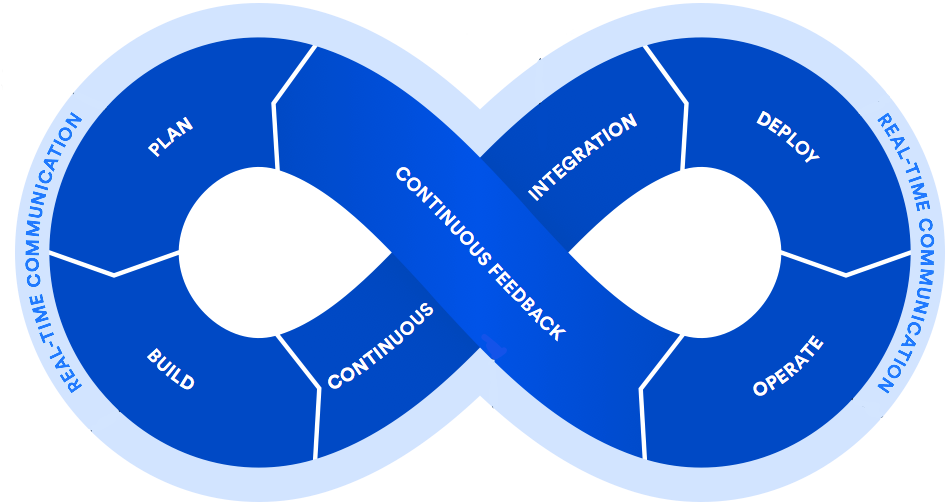
\includegraphics[scale=0.38]{images/devops.png}

\end{frame}

% ----------------------------------------------------------------------------------

\begin{frame}{Mission du DevOps : Intégration continue et déploiement continu (CI/CD)}

\centering
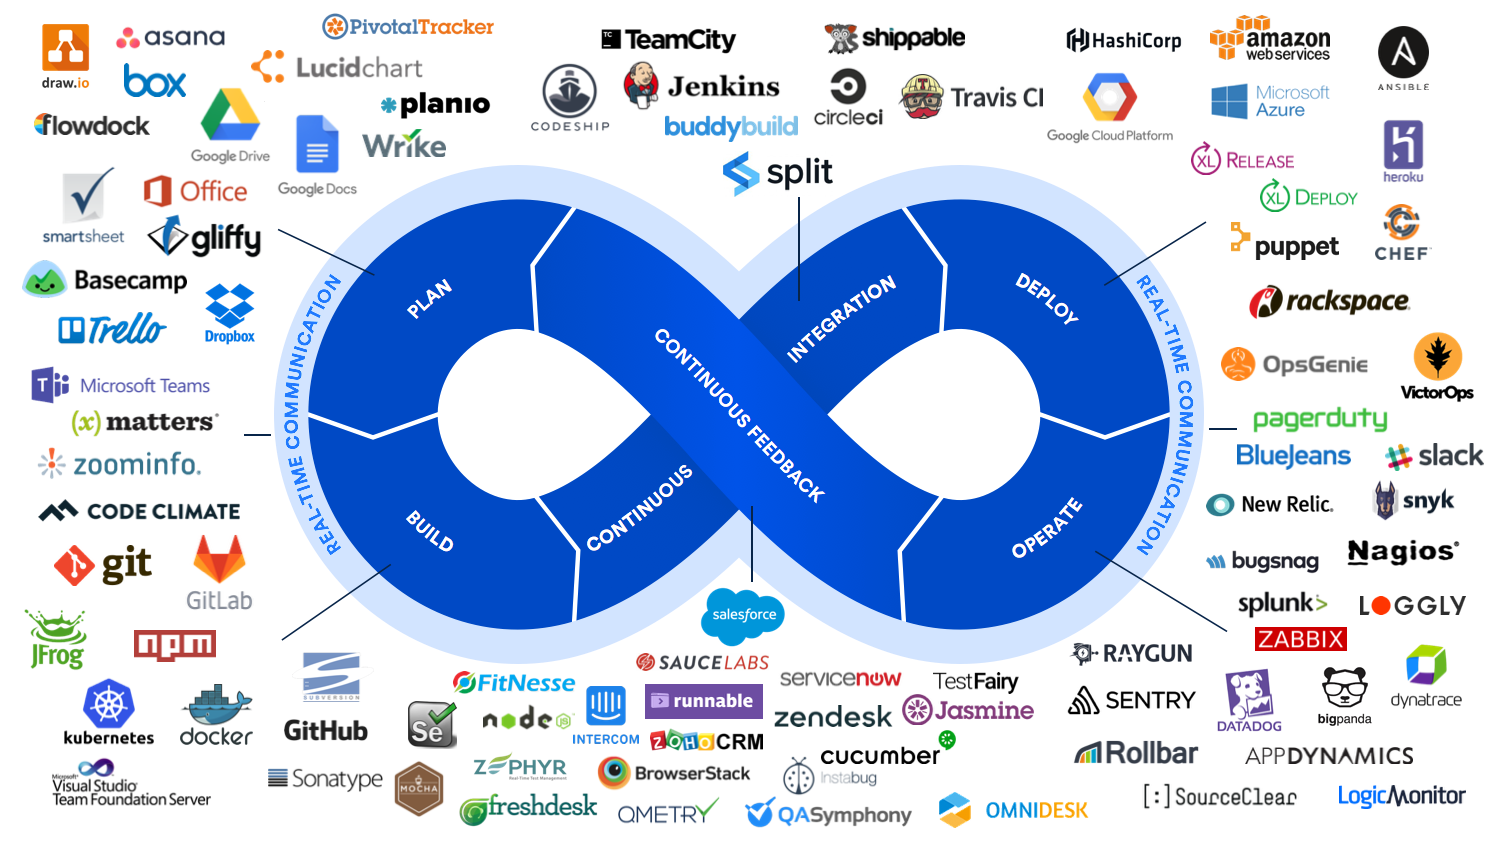
\includegraphics[scale=0.69]{images/devopstool.png}

\end{frame}

% ----------------------------------------------------------------------------------

\begin{frame}{Roadmap}
\centering
\large
\url{https://roadmap.sh/devops} 
 
\end{frame}

% ----------------------------------------------------------------------------------

\section{Infrastructure-as-code}

% ----------------------------------------------------------------------------------

\begin{frame}{Architecture orientée services (SOA)}

    \begin{alertblock}<1->{Définition}
      \begin{itemize}
        \item \textbf{Approche d’architecture logicielle} organisée autour de \textbf{services}.
        \item Un service = une \textbf{fonctionnalité autonome} exposée via une interface standard.
        \item Communication via des protocoles réseau (SOAP, REST, gRCP/RMI, messages).
      \end{itemize}
    \end{alertblock}

    \begin{alertblock}<2->{Principes}
      \begin{itemize}
        \item \textbf{Réutilisabilité} : services mutualisés dans plusieurs applications.
        \item \textbf{Interopérabilité} : indépendants des langages et plateformes.
        \item \textbf{Faible couplage} : évolution indépendante des services.
        \item \textbf{Composition} : services combinés pour former des processus métiers.
      \end{itemize}
    \end{alertblock}

\end{frame}

% ----------------------------------------------------------------------------------

\begin{frame}{SOA dans le Cloud}

    \begin{alertblock}<1->{Utilisation dans le cloud}
      \begin{itemize}
        \item Les services sont \textbf{déployés et consommés à la demande}.
        \item Mise en œuvre via des \textbf{APIs exposées en ligne}.
        \item Intégration fréquente avec des \textbf{microservices} et du \textbf{serverless}.
        \item Supportée par des \textbf{plateformes cloud} (\emph{providers}) : AWS, Azure, GCP.
      \end{itemize}
    \end{alertblock}

    \begin{alertblock}<2->{Avantages pour le cloud}
      \begin{itemize}
        \item \textbf{Élasticité} : montée en charge dynamique des services.
        \item \textbf{Scalabilité mondiale} : services accessibles partout.
        \item \textbf{Agilité accrue} : déploiement rapide de nouveaux services.
        \item \textbf{Coût à l’usage} : facturation en fonction de la consommation.
      \end{itemize}
    \end{alertblock}

\end{frame}

% ----------------------------------------------------------------------------------

\begin{frame}{Réalité: Des Deathstars}
\centering
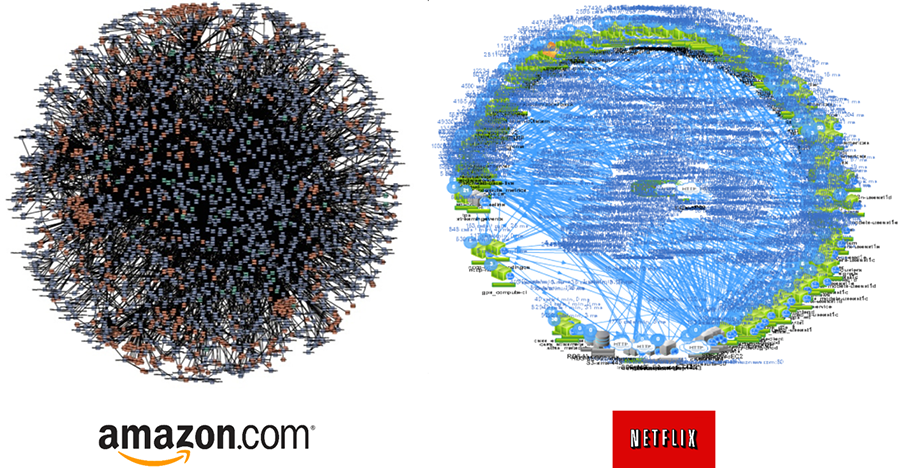
\includegraphics[scale=0.4]{figures/deathstar.png}

\end{frame}

% ----------------------------------------------------------------------------------

\begin{frame}{Déployer et maintenir des applications}

\begin{alertblock}{Que faut-il faire ?}
  \begin{itemize}
    \item Préparer \textbf{ses services} pour fonctionner \textbf{de façon atomique}
    \item Préparer \textbf{ses ressources} (n\oe uds physiques/virtuels, VM/containers, 
          réseau, règles de sécurité, secrets/identités).
    \item \textbf{Installer, configurer et démarrer} les services sur ces ressources .
    \item \textbf{Adapter l’infrastructure} aux événements : autoscaling, auto-healing, etc.
  \end{itemize}
\end{alertblock}

\end{frame}
% ----------------------------------------------------------------------------------

\begin{frame}{Déployer et maintenir des applications}

\begin{alertblock}{Challenges}
  \begin{itemize}
    \item \textbf{Gérer les dépendances} : induit un ordre partiel sur les opérations
    \item \textbf{Déployer sans faute} : Avoir des opérations de déploiement atomiques (déployer, mise à jour, supprimer) sûres.
    \item \textbf{Robustesse} : tolérance aux pannes, passage à l'échelle, rollbacks rapides, etc.
    \item \textbf{Sécurité} : secrets/identités, durcissement, moindre privilège, conformité.
    \item \textbf{Impact} : coûts, empreinte carbone, dette opérationnelle, incidents clients.
  \end{itemize}
\end{alertblock}

\end{frame}


% ----------------------------------------------------------------------------------

\begin{frame}{Gérer les dépendances}

\begin{center}
\begin{tikzpicture}
    \node[] (n) {Notation : };
    % \node[step] (commit) {Commit Code};
    \node[draw, rectangle, right=0cm of n, minimum width=2cm, minimum height=0.8cm] (s1) {Service 1 }; 
    \node[draw, rectangle, minimum width=2cm, minimum height=0.8cm, right=1cm of s1] (s2) {Service 2}; 
    \simpleprovideuse{s1}{s2}
    \node[below=0.3cm of s1, xshift=1cm] (t) {
    \begin{tabular}{c}
    Dans ce cas, Service 1 expose son API, qui est utilisée par Service 2.\\
    Service 1 fournit des informations, un service, etc. via son port.\\
    On parle de \emph{provide port} pour Service 1 et de \emph{use port} pour Service 2
    \end{tabular} }; 
\end{tikzpicture}
\end{center}

\begin{columns}[T,onlytextwidth]
    \begin{column}{.6\linewidth}
      \begin{tikzpicture}
    \node[draw, rectangle, minimum width=2cm, minimum height=0.8cm] (s1) {\bf S1}; 
    \node[draw, rectangle, minimum width=2cm, minimum height=0.8cm, right=1cm of s1] (s2) {\bf S2}; 
    \node[draw, rectangle, minimum width=2cm, minimum height=0.8cm, right=1cm of s2] (s3) {\bf S3}; 
    \node[draw, rectangle, minimum width=2cm, minimum height=0.8cm, below=1cm of s2, xshift=-1cm] (s4) {\bf S4}; 
    \node[draw, rectangle, minimum width=2cm, minimum height=0.8cm, right=1cm of s4] (s5) {\bf S5}; 

    \simpleprovideuse{s1}{s2}
    \simpleprovideuse{s2}{s3}
    \simpleprovideuse{s1}{s4}
    \simpleprovideuse{s2}{s5}
    \simpleprovideuse{s5}{s4}

\end{tikzpicture} 
    \end{column}
    \begin{column}{.4\linewidth}
    \vspace{-0.1in}
      \begin{alertblock}{Dépendances}
        \begin{itemize}
          \item {\bf S2} dépend de {\bf S1}
          \item {\bf S3} dépend de {\bf S2}
          \item {\bf S4} dépend de {\bf S1} et {\bf S5}
          \item {\bf S5} dépend de {\bf S2}
        \end{itemize}
      \end{alertblock}
    \end{column}
  \end{columns}

\end{frame}

% ----------------------------------------------------------------------------------

\begin{frame}{Déployer sans faute}

\begin{columns}[T,onlytextwidth]
    \begin{column}{.6\linewidth}
      \begin{tikzpicture}
    % \node[step] (commit) {Commit Code};
    \node[draw, rectangle, minimum width=2cm, minimum height=0.8cm] (s1) {\bf S1};
    \node[draw, rectangle, minimum width=2cm, minimum height=0.8cm, right=1cm of s1] (s2) {\bf S2}; 
    \node[draw, rectangle, minimum width=2cm, minimum height=0.8cm, right=1cm of s2] (s3) {\bf S3}; 
    \node[draw, rectangle, minimum width=2cm, minimum height=0.8cm, below=1cm of s2, xshift=-1cm] (s4) {\bf S4}; 
    \node[draw, rectangle, minimum width=2cm, minimum height=0.8cm, right=1cm of s4] (s5) {\bf S5}; 

    \simpleprovideuse{s1}{s2}
    \simpleprovideuse{s2}{s3}
    \simpleprovideuse{s1}{s4}
    \simpleprovideuse{s2}{s5}
    \simpleprovideuse{s5}{s4}
    
    \node[draw, circle, minimum width=0.5cm, right=-0.5cm of s1, yshift=-0.4cm, fill=green] (o1) {\small\bf 1}; 
    \node[draw, circle, minimum width=0.5cm, right=-0.5cm of s2, yshift=-0.4cm, fill=green] (o2) {\small\bf 2}; 
    \node[draw, circle, minimum width=0.5cm, right=-0.5cm of s3, yshift=-0.4cm, fill=green] (o3) {\small\bf 3}; 
    \node[draw, circle, minimum width=0.5cm, right=-0.5cm of s4, yshift=-0.4cm, fill=green] (o4) {\small\bf 3}; 
    \node[draw, circle, minimum width=0.5cm, right=-0.5cm of s5, yshift=-0.4cm, fill=green] (o5) {\small\bf 4}; 

\end{tikzpicture} 
    \end{column}
    \begin{column}{.4\linewidth}
    \vspace{-0.1in}
      \begin{alertblock}{Relation d'ordre partiel strict}
        \begin{itemize}
            \item Deploy {\bf S1} $>$ Deploy {\bf S2}
            \item Deploy {\bf S2} $>$ Deploy {\bf S3}
            \item Deploy {\bf S2} $>$ Deploy {\bf S5}
            \item Deploy {\bf S4} $>$ Deploy {\bf S1}
            \item Deploy {\bf S4} $>$ Deploy {\bf S5}
        \end{itemize}
      \end{alertblock}
    \end{column}
  \end{columns}
   
\vspace{0.1cm}
   
Exemple de trace: Deploy {\bf S1}; Deploy {\bf S2}; Deploy {\bf S5}; Deploy {\bf S4}; Deploy {\bf S3};

    \vspace{0.3cm}

  \begin{exampleblock}{Rappel}
    \begin{itemize}
      \item \textbf{Irréflexivité} : $\forall a \in E,\; \neg(a < a)$
      \item \textbf{Transitivité} : $\forall a,b,c \in E,\; (a < b \land b < c) \;\Rightarrow\; a < c$
      \item \textbf{Asymétrie} : $\forall a,b \in E,\; (a < b) \;\Rightarrow\; \neg(b < a)$
    \end{itemize}
  \end{exampleblock}
\end{frame}

% ----------------------------------------------------------------------------------

\begin{frame}{Replace sans faute}
\vspace{-0.5cm}
    \begin{center}
    \begin{tikzpicture}

    % \node[step] (commit) {Commit Code};
    \node[draw, rectangle, minimum width=2cm, minimum height=0.8cm] (s1) {\bf S1}; 
    \node[draw, rectangle, minimum width=2cm, minimum height=0.8cm, right=1cm of s1] (s2) {\bf S2}; 
    \node[draw, rectangle, minimum width=2cm, minimum height=0.8cm, right=1cm of s2] (s3) {\bf S3}; 
    \node[draw, rectangle, minimum width=2cm, minimum height=0.8cm, below=1cm of s2, xshift=-1cm] (s4) {\bf S4}; 
    \node[draw, rectangle, minimum width=2cm, minimum height=0.8cm, right=1cm of s4] (s5) {\bf S5}; 

    \simpleprovideuse{s1}{s2}
    \simpleprovideuse{s2}{s3}
    \simpleprovideuse{s1}{s4}
    \simpleprovideuse{s2}{s5}
    \simpleprovideuse{s5}{s4}

    \node[left=0.2cm of s1] (sc1) {
    \begin{tabular}{l}
        Scenario: Replace {\bf S2} \\ 
        C'est à dire : Destroy {\bf S2} ;  Deploy {\bf S2}
    \end{tabular}};
    
\end{tikzpicture} 
    \end{center}

\begin{columns}[T,onlytextwidth]
    \begin{column}{.45\linewidth}
      \begin{alertblock}{Deploy}
        \begin{itemize}
            \item Deploy {\bf S1} $>$ Deploy {\bf S2}
            \item Deploy {\bf S2} $>$ Deploy {\bf S3}
            \item Deploy {\bf S2} $>$ Deploy {\bf S5}
            \item Deploy {\bf S4} $>$ Deploy {\bf S1}
            \item Deploy {\bf S4} $>$ Deploy {\bf S5}
        \end{itemize}
      \end{alertblock}
    \end{column}
    \begin{column}{.45\linewidth}
    
      \begin{alertblock}{Destroy}
        \begin{itemize}
            \item Destroy {\bf S1} $<$ Destroy {\bf S2}
            \item Destroy {\bf S1} $<$ Destroy {\bf S4}
            \item Destroy {\bf S2} $<$ Destroy {\bf S3}
            \item Destroy {\bf S2} $<$ Destroy {\bf S5}
            \item Destroy {\bf S5} $<$ Destroy {\bf S4}
        \end{itemize}
      \end{alertblock}
    \end{column}
  \end{columns}

\end{frame}

% ----------------------------------------------------------------------------------

\begin{frame}{Replace sans faute: Graphe de dépendance}
$\forall${\bf S}, Replace {\bf S} := Destroy {\bf S}; Deploy {\bf S}
\vspace{-0.1in}
\begin{columns}[T,onlytextwidth]
    \begin{column}{.4\linewidth}
      \begin{alertblock}{Destroy}
  \begin{itemize}
    \item \small Destroy {\bf S1} $<$ Destroy {\bf S2}
    \item \alert<2>{\small Destroy {\bf S2} $<$ Destroy {\bf S3}}
    \item \alert<2>{\small Destroy {\bf S2} $<$ Destroy {\bf S5}}
    \item \alert<3>{\small Destroy {\bf S5} $<$ Destroy {\bf S4}}
    \item \small Destroy {\bf S1} $<$ Destroy {\bf S4}
  \end{itemize}
\end{alertblock}
\vspace{-0.05in}
\begin{alertblock}{Deploy}
  \begin{itemize}
    \item \small Deploy {\bf S1} $>$ Deploy {\bf S2}
    \item \alert<4>{\small Deploy {\bf S2} $>$ Deploy {\bf S3}}
    \item \alert<4>{\small Deploy {\bf S2} $>$ Deploy {\bf S5}}
    \item \alert<5>{\small Deploy {\bf S5} $>$ Deploy {\bf S4}}
    \item \small Deploy {\bf S4} $>$ Deploy {\bf S1}
  \end{itemize}
\end{alertblock}

    \end{column}
    
    \begin{column}{.5\linewidth}
     \vspace{-0.3cm}
      \begin{tikzpicture}

% -----------------------
\onslide<1->{
\node[](des2){Destroy \textbf{S2}};
\node[below=0.5cm of des2](dep2){Deploy \textbf{S2}};

\draw[-{Stealth[scale=1.0]}] (des2) -- (dep2);
}
\onslide<1>{
\node[rectangle, draw, inner sep=2.5pt, fit=(des2) (dep2) ](rep2){};
\node[left=0cm of rep2](repL2){Replace \textbf{S2}};
}

% -----------------------
\onslide<2>{
    \node[above=0.7cm of des2, xshift=-1.5cm](des3){\alert{Destroy \textbf{S3}}};
    \node[above=0.7cm of des2, xshift=1.5cm](des5){\alert{Destroy \textbf{S5}}};
}
\onslide<2->{
\draw[-{Stealth[scale=1.0]}] (des3) -- (des2);
\draw[-{Stealth[scale=1.0]}] (des5) -- (des2);
}
\onslide<3->{
    \node[above=0.7cm of des2, xshift=-1.5cm](des3){Destroy \textbf{S3}};
    \node[above=0.7cm of des2, xshift=1.5cm](des5){Destroy \textbf{S5}};
}
% -----------------------
\onslide<3>{
\node[above=0.65cm of des5](des4){\alert{Destroy \textbf{S4}}};
\draw[-{Stealth[scale=1.0]}] (des4) -- (des5);
}
\onslide<3->{
\draw[-{Stealth[scale=1.0]}] (des4) -- (des5);
}
\onslide<4->{
\node[above=0.65cm of des5](des4){Destroy \textbf{S4}};
\draw[-{Stealth[scale=1.0]}] (des4) -- (des5);
}
% -----------------------
\onslide<4>{
\node[below=0.7cm of dep2, xshift=-1.5cm](dep3){\alert{Deploy \textbf{S3}}};
\node[below=0.7cm of dep2, xshift=1.5cm](dep5){\alert{Deploy \textbf{S5}}};
}
\onslide<4->{
\draw[-{Stealth[scale=1.0]}] (dep2) -- (dep3);
\draw[-{Stealth[scale=1.0]}] (dep2) -- (dep5);
}
\onslide<5->{
\node[below=0.7cm of dep2, xshift=-1.5cm](dep3){Deploy \textbf{S3}};
\node[below=0.7cm of dep2, xshift=1.5cm](dep5){Deploy \textbf{S5}};
}
% -----------------------
\onslide<5>{
\node[below=0.65cm of dep5](dep4){\alert{Deploy \textbf{S4}}};
}
\onslide<5->{
\draw[-{Stealth[scale=1.0]}] (dep5) -- (dep4);
}
\onslide<6->{
\node[below=0.65cm of dep5](dep4){Deploy \textbf{S4}};
}
% -----------------------
\onslide<6->{

\node[draw, dotted, thin, fit=(des4) (dep4) (des3)](graph){};
\node[below=0.2cm of graph](graphL){Graphe de dépendance pour Replace \textbf{S2}};

}

\end{tikzpicture}
    \end{column}
  \end{columns}

\end{frame}

% ----------------------------------------------------------------------------------

\begin{frame}{Robustesse et Sécurité}

\begin{center}
\begin{tikzpicture}

    \node[draw, rectangle, minimum width=2cm, minimum height=0.8cm] (s1) {\bf S1}; 
    \node[draw, rectangle, minimum width=2cm, minimum height=0.8cm, right=1cm of s1] (s2) {\bf S2}; 
    \node[draw, rectangle, minimum width=2cm, minimum height=0.8cm, right=1cm of s2] (s3) {\bf S3}; 
    \node[draw, rectangle, minimum width=2cm, minimum height=0.8cm, below=1cm of s2, xshift=-1cm] (s4) {\bf S4}; 
    \node[draw, rectangle, minimum width=2cm, minimum height=0.8cm, right=1cm of s4] (s5) {\bf S5}; 

    \simpleprovideuse{s1}{s2}
    \simpleprovideuse{s2}{s3}
    \simpleprovideuse{s1}{s4}
    \simpleprovideuse{s2}{s5}
    \simpleprovideuse{s5}{s4}

    \node[left=2cm of s1](s0){}; 
    \draw[-{Stealth[scale=2.0]}, double, line width=1pt, double distance=1pt](s0) -- (s1); 

\end{tikzpicture}
\end{center}

\begin{alertblock}{Robustesse}
  \begin{itemize}
    \item \textbf{Déclencheur} : Un service (e.g., S2) tombe
    \item \textbf{Action} : Ce service est remplacé
  \end{itemize}
\end{alertblock}

\begin{alertblock}{Sécurité}
  \begin{itemize}
    \item L'utilisateur n'a accès qu'au service façade (e.g., S1)
    \item Les services permettent d'utiliser JRMP (Java Remote Method Protocol) entre eux
  \end{itemize}
\end{alertblock}

\end{frame}

% ----------------------------------------------------------------------------------

\begin{frame}{Impact}

\begin{alertblock}{Élaborer des stratégies}
Pour avoir des impactes
  \begin{itemize}
    \item Qualité de service (DevOps)
    \item Financier (FinOps)
    \item Sécurité (SecOps)
    \item Énergétique (GreenOps)
  \end{itemize}
\end{alertblock}

\end{frame}

% ----------------------------------------------------------------------------------

\begin{frame}{Impact}

\begin{alertblock}{Exemple}
Une migration d'une partie de l'infrastructure
  \begin{enumerate}
    \item[1] Garder deux environnements et basculer progressivement les services.
    \item[$\Rightarrow$] Coûteux financièrement mais assure une continuité de service
    \item[2] Supprimer l'ancien environnement progressivement et remplacer les resources au fur et à mesure
    \item[$\Rightarrow$] Peu réduire le coût financier et énergétique au prix d'une interruption de service
  \end{enumerate}
\end{alertblock}

\end{frame}

% ----------------------------------------------------------------------------------

\begin{frame}{Déployer et maintenir des applications}

\begin{alertblock}{Challenges}
  \begin{itemize}
    \item \textbf{Gérer les dépendances} : induit un ordre partiel sur les opérations
    \item \textbf{Déployer sans faute} : Avoir des opérations de déploiement atomiques (déployer, mise à jour, supprimer) sûres.
    \item \textbf{Robustesse} : tolérance aux pannes, passage à l'échelle, rollbacks rapides, etc.
    \item \textbf{Sécurité} : secrets/identités, durcissement, moindre privilège, conformité.
    \item \textbf{Impact} : coûts, empreinte carbone, dette opérationnelle, incidents clients.
    \item[$\Rightarrow$] \color{red} \textbf{Automatiser} avec l'\textbf{infrastructure-as-code}
  \end{itemize}
\end{alertblock}

\end{frame}
% ----------------------------------------------------------------------------------
\begin{frame}{Infrastructure as Code (IaC)}

  \begin{alertblock}{Définition}
    \begin{itemize}
      \item \textbf{Infrastructure as Code} = pratique consistant à 
      \textbf{décrire et gérer l’infrastructure (réseau, serveurs, VM, containers, règles)} 
      au moyen de code en utilisant
    \begin{itemize}
      \item des \textbf{langages génériques}, ou GPL (General Purpose Language), avec des bibliothèques
      \item des \textbf{langages dédiés}, ou DSL (Domain Specific Language)
      \item des \textbf{langages de configuration} (YAML ou JSON par exemple)
    \end{itemize}
      \item L’infrastructure est donc \textbf{déclarative et reproductible}, plutôt que créée manuellement.
    \end{itemize}
  \end{alertblock}
\end{frame}

% ----------------------------------------------------------------------------------

\begin{frame}{IaC et DevOps : comment ça marche ?}

  \begin{alertblock}{Dans la pratique}
    \begin{itemize}
      \item Le code d’infrastructure est \textbf{stocké dans Git}, versionné comme le code applicatif.
      \item Les outils (Terraform, Ansible, Pulumi, CloudFormation, etc.) 
            \textbf{appliquent le code} pour provisionner ou mettre à jour les ressources.
      \item Intégration dans les \textbf{pipelines CI/CD} : validation, tests, déploiement automatisé.
      \item Résultat : la création/évolution de l’infra suit le même cycle que le code des Devs 
     \item[] \textit{plan → review → merge → apply}
    \end{itemize}
  \end{alertblock}

\end{frame}

% ----------------------------------------------------------------------------------
% ----------------------------------------------------------------------------------

\begin{frame}{IaC et DevOps : comment ça marche ?}

  \begin{tikzpicture}[auto, node distance=1cm, scale=0.5]

% DevOps fig + txt
\node[yshift=0.5cm] (ldevops) {\LARGE \faMale};
\node[left=-0.1cm of ldevops] (rdevops) {\LARGE \faFemale};
\node[fit=(ldevops) (rdevops), inner sep=1pt] (sdevops) {};
\node[below=0 of sdevops] (devops) {DevOps};
\node[fit=(sdevops) (devops), inner sep=1pt] (blockdevops) {};

% Conflang
\node[draw, rectangle, rounded corners=5pt, right=1.3cm of blockdevops] (conflang) {\begin{tabular}{c}GPL; DSL\\Language de\\configuration\end{tabular}};
\node[above=-0.25cm of conflang, xshift=18pt](midconflang){};

% Target and current infra
\node[draw, rectangle, right=1.5cm of conflang, minimum height=1.4cm] (targetinfra) {\begin{tabular}{c}
Infrastructure\\Ciblée\end{tabular}};
\node[draw, rectangle, right=0.5cm of targetinfra, minimum height=1.4cm] (currentinfra) {\begin{tabular}{c}
Infrastructure\\Courante
\end{tabular}};
\node[fit=(targetinfra) (currentinfra), inner sep=1pt] (blockinfra) {};

% Ressources

% Reconciliation
\node[draw, rectangle, rounded corners=10pt, below=0.8cm of blockinfra] (reconciliation){\begin{tabular}{l}
Réconciliation d'état \\ 
$\bullet$ Différence (quand stateful) \\ 
$\bullet$ Planifie la reconf. \\ 
$\bullet$ Exécute
\end{tabular}};

% New infra
\node[draw, rectangle, left=1.3cm of reconciliation, minimum height=0.7cm, minimum width=2cm] (newinfra) {\begin{tabular}{c}
Nouvelle\\Infrastructure
\end{tabular}};


% Arrows
\draw[-{Stealth[length=2mm]}, thick, line width=0.4mm] (blockdevops) -- node {utilise} (conflang);
\draw[-{Stealth[length=2mm]}, thick, line width=0.4mm] (conflang) -- node [above] {décrit} (targetinfra);

% \draw[-{Stealth[length=2mm]}, thick, line width=0.4mm] (conflang.north) -- node [below] {dirige, modifie} (currentinfra.north);

\draw[-{Stealth[length=2mm]}, thick, line width=0.4mm]
  (conflang.north) -- ++(0,0.7)
  -- node[above] {dirige, modifie} ++(14.5,0)
  -- (currentinfra.north);


\draw[-{Stealth[length=2mm]}, thick, line width=0.4mm](targetinfra)-- node [xshift=0.4cm, yshift=-0.3cm] {input} (reconciliation);
\draw[-{Stealth[length=2mm]}, thick, line width=0.4mm](currentinfra)-- (reconciliation);
\draw[-{Stealth[length=2mm]}, thick, line width=0.4mm](reconciliation)-- node {output} (newinfra);

\end{tikzpicture}


\end{frame}

% ----------------------------------------------------------------------------------

\begin{frame}{Les rôles des outils d'IaC}

\hspace*{-0.7cm}
\begin{tikzpicture}

    % \node[] (commit) {Commit Code};

\node[] (packaging) {
    \begin{tabular}{c}
    \textbf{Management}\\
    \textbf{d'application}
    \end{tabular}
    };
\node[below=0cm of packaging] (packagingL) {
    \begin{tabular}{c}
    \small Customiser, configurer\\
    \small tester l'application\\
    \small et la conteneuriser\\
    \small 
    \end{tabular}
};
\node[right=0.8cm of packaging] (provisioning) {
    \begin{tabular}{c}
    \textbf{Provisionnement} \\ 
    \textbf{d'infrastructure}
    \end{tabular}
};
\node[below=0cm of provisioning] (provisioningL) {
    \begin{tabular}{c}
    \small Demander ressources\\
    \small physiques ou virtuelles;\\
    \small configurer le réseau;\\
    \small et règles sécurité
    \end{tabular}
};
    
\node[right=0.8cm of provisioning] (configmanagement) {
    \begin{tabular}{c}
    \textbf{Installation et}\\
    \textbf{Configuration}
    \end{tabular}
};
\node[below=0cm of configmanagement] (configmanagementL) {
    \begin{tabular}{c}
    \small Installer les services\\
    \small (app + deps)\\
    \small configurer les services;\\
    \small et les intégrer
    \end{tabular}
};

    % -------

\node[right=0.8cm of configmanagement] (orchestration) {
\begin{tabular}{c}
\textbf{Orchestration}\\
\textbf{de cycle de vie}
\end{tabular}
};
\node[below=0cm of orchestration] (orchestrationL) {
\begin{tabular}{c}
\small Upgrades auto;\\
\small Backup et recovery;\\
\small Surveillance;\\
\small Passage à l'échelle
\end{tabular}
};

\node[rectangle, draw, fit=(provisioning) (provisioningL), dkblue, line width=2pt](){};
    
\end{tikzpicture}

\end{frame}

\begin{frame}{Les rôles des outils d'IaC... Dans un exemple concret}

On veut une \textbf{base de données maitre}, et \textbf{des réplicats} de cette base de données. Ces services sont chacun sur \textbf{une VM différente, sur un noeud différent}. Cependant, tous ces \textbf{noeuds sont connecté en réseau}. Dans le cas où un \textbf{réplicat tombe en panne, il faut en redéployer} un.

\vspace*{0.7cm}

\hspace*{-0.7cm}
\begin{tikzpicture}


\onslide<1>{}

\onslide<2->{
    \node[] (packaging) {
    \begin{tabular}{c}
    \textbf{Management}\\
    \textbf{d'application}
    \end{tabular}
    };

     \node[right=0.8cm of packaging] (provisioning) {
    \begin{tabular}{c}
    \textbf{Provisionnement} \\ 
    \textbf{d'infrastructure}
    \end{tabular}
    };

    \node[right=0.8cm of provisioning] (configmanagement) {
    \begin{tabular}{c}
    \textbf{Installation et}\\
    \textbf{Configuration}
    \end{tabular}
    };

   \node[right=0.8cm of configmanagement] (orchestration) {
    \begin{tabular}{c}
    \textbf{Orchestration}\\
    \textbf{de cycle de vie}
    \end{tabular}
    };
}

    
\onslide<3->{
    \node[below=0cm of packaging] (packagingL) {
    \begin{tabular}{c}
    \small Créer un conteneur\\ 
    \small (Docker) pour démarrer\\
    \small une base de données\\
    \end{tabular}
    };
    

}

    
\onslide<4->{

   
    \node[below=0cm of provisioning] (provisioningL) {
    \begin{tabular}{c}
    \small Créer un VPC (subnet);\\ 
    \small Demander des noeuds;\\ 
    \small Définir des VMs / cluster;\\ 
    \small Firewall\\ 
    \end{tabular}
    };
    

}

    
\onslide<5->{
    
    \node[below=0cm of configmanagement] (configmanagementL) {
    \begin{tabular}{c}
    \small Démarrer les conteneurs\\
    \small sur les VMs; configurer \\
    \small et boostrapper les BDDs; \\
    \small intégrer master et réplicats \\
    \end{tabular}
    };

}
    
\onslide<6->{

    \node[below=0cm of orchestration] (orchestrationL) {
    \begin{tabular}{c}
    \small Configurer un trigger:\\
    \small détecter une panne\\
    \small Configurer une action:\\
    \small rédeployer une BDD\\
    \end{tabular}
    };
  
} 
    
    
\end{tikzpicture}

\end{frame}


\begin{frame}{Les rôles des outils d'IaC... Dans une cuisine ?}

\hspace*{-0.7cm}
\begin{tikzpicture}

    % \node[] (commit) {Commit Code};
    
    \node[] (packaging) {
    \begin{tabular}{c}
    \textbf{Management}\\
    \textbf{d'application}
    \end{tabular}
    };
    \node[below=0cm of packaging] (packagingL) {
    \begin{tabular}{c}
    \small Former les cuisiniers: \\
    \small leur apprendre des\\
    \small recettes, etc.\\
    \end{tabular}
    };
    
    % ----------

    \node[right=0.8cm of packaging] (provisioning) {
    \begin{tabular}{c}
    \textbf{Provisionnement} \\ 
    \textbf{d'infrastructure}
    \end{tabular}
    };
    \node[below=0cm of provisioning] (provisioningL) {
    \begin{tabular}{c}
    \small Fourni plan de travail,\\ 
    \small robots de cuisine,\\ 
    \small four, etc. et les\\ 
    \small assembler.\\ 
    \end{tabular}
    };
    
    % ----------

    \node[right=0.8cm of provisioning] (configmanagement) {
    \begin{tabular}{c}
    \textbf{Installation et}\\
    \textbf{Configuration}
    \end{tabular}
    };
    \node[below=0cm of configmanagement] (configmanagementL) {
    \begin{tabular}{c}
    \small Assigner les cuisiniers\\
    \small à des postes, et à des\\
    \small taches; leur donner des\\
    \small outils de coms; etc.
    \end{tabular}
    };

    % -------

    \node[right=0.8cm of configmanagement] (orchestration) {
    \begin{tabular}{c}
    \textbf{Orchestration}\\
    \textbf{de cycle de vie}
    \end{tabular}
    };
    \node[below=0cm of orchestration] (orchestrationL) {
    \begin{tabular}{c}
    \small Avoir un chef de brigade\\
    \small prêt à changer l'organisation\\
    \small pour plus d'efficacité, ou\\
    \small répondre à un imprévu\\
    \end{tabular}
    };
   
    
    
\end{tikzpicture}

\begin{center}
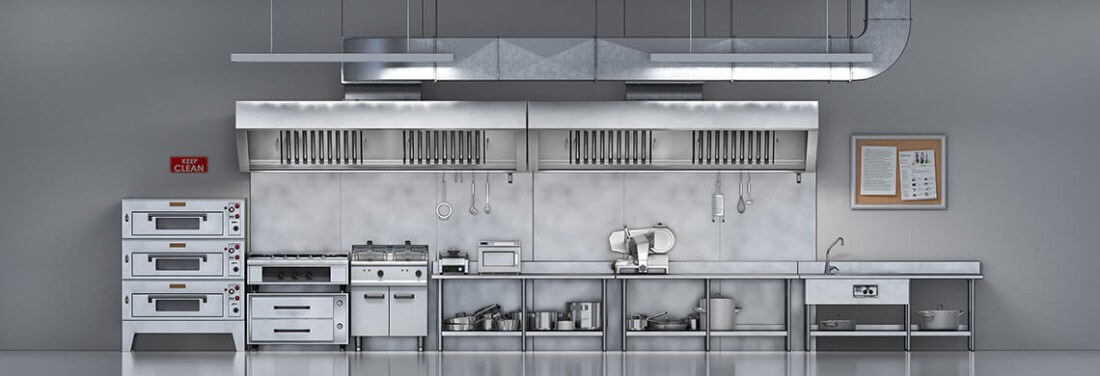
\includegraphics[scale=0.25]{images/Vue-cuisine-3D-face-cuisson-pano-1634649966.jpg}
\end{center}

\end{frame}

% ----------------------------------------------------------------------------------
\begin{frame}{Atouts de l’Infrastructure as Code}

  \begin{alertblock}{Pourquoi adopter l’IaC ?}
    \begin{itemize}
      \item \textbf{Interopérable} : fonctionne sur multi-cloud et on-premise.
      \item \textbf{Réutilisable} : modules et templates factorisables.
      \item \textbf{Versionnable} : suivi dans Git, rollback possible.
      \item \textbf{Automatisable} : intégré aux pipelines CI/CD.
      \item \textbf{Traçable et auditable} : chaque changement est explicite.
      \item \textbf{Scalable et idempotent} : état final garanti, même à grande échelle.
      \item \textbf{Auto-documentant} : le code décrit l’infrastructure.
    \end{itemize}
  \end{alertblock}

\end{frame}

% ----------------------------------------------------------------------------------
\begin{frame}{Technologie d’Infrastructure as Code}

\begin{table}[H]
    \centering
    \resizebox{0.85\textwidth}{!}{
    \begin{tabular}{|c|c|c|c|}
\hline
\textbf{Technology} & \textbf{Provisioning} & \textbf{Conf. Mgmt} & \textbf{Orchestration}\\ \hline
Ansible & \OKmark & \OKOKmark & \KOmark \\ 
AWS + CloudFormation (CFN)  & \OKOKmark & \KOmark & \OKmark\\ 
Azure Resource Manager (ARM) & \OKOKmark & \KOmark & \OKmark \\ 
CFEngine & \OKmark & \OKOKmark & \KOmark \\ 
Chef & \OKmark & \OKOKmark & \KOmark \\ 
Google's Infrastructure manager & \OKOKmark & \KOmark & \OKmark\\ 
OpenStack + Heat & \OKOKmark & \KOmark & \OKmark\\ 
Juju  & \OKOKmark & \OKOKmark & \OKOKmark \\
Kubernetes + Manifest & \OKOKmark & \KOmark & \OKOKmark\\ 
Nomad & \OKOKmark & \KOmark & \OKOKmark \\ %
Pulumi & \OKOKmark & \OKmark & \KOmark\\ % Idem Terraform avec langage généraliste. Provision + scripts init. 
Puppet & \OKmark & \OKOKmark & \KOmark \\ % Config déclarative
SaltStack & \OKmark & \OKOKmark & \KOmark \\ %
Terraform & \OKOKmark & \OKmark & \KOmark \\
TOSCA & \OKOKmark & \OKOKmark  & \OKOKmark \\ 
\hline
\end{tabular}
}
\end{table}

\end{frame}


% ----------------------------------------------------------------------------------

\begin{frame}{En résumé}

\begin{alertblock}{Intégration continue / Déploiement continue (CI/CD)}
  \begin{itemize}
        \item \textbf{CI} : build + tests à chaque commit.
      \item \textbf{CD} : déploiement automatisé 
  \end{itemize}
\end{alertblock}

\begin{alertblock}{DevOps}
  \begin{itemize}
    \item Dev = \textbf{garant de l’évolution du service} (innovation, nouvelles fonctionnalités, correction de bugs, qualité logicielle)
    \item Ops = \textbf{garant de la continuité de service} (disponibilité, robustesse, supervision), en lien étroit avec les Devs
  \end{itemize}
\end{alertblock}


\end{frame}

% ----------------------------------------------------------------------------------

\begin{frame}{En résumé}

\begin{alertblock}{Architecture orientée services (SOA)}
  \begin{itemize}
    \item Approche modulaire: un service = une fonctionnalité
    \item Utilisation d'API pour composer
    \item Difficile à gérer à cause de la taille
  \end{itemize}
\end{alertblock}

\begin{alertblock}{Infrastructure-as-code}
  \begin{itemize}
    \item Solution pour déployer sous forme de code
    \begin{itemize}
        \item Préparer son application (conteneurisation)
        \item Préparer ses ressources (provisionnement)
        \item Installer son application (gestion de configuration)
        \item Installer son application (orchestration)
    \end{itemize}
    \item Interopérable, réutilisable, versionnable, automatisable, idempotent
  \end{itemize}
\end{alertblock}

\end{frame}

% ----------------------------------------------------------------------------------

\begin{frame}
\begin{figure}
    \centering
    \begin{tikzpicture}

\node[draw, rectangle, rounded corners=8, minimum height=1.3cm] (package) {
\begin{tabular}{c}
Build \\ packaging     
\end{tabular}
};

\node[draw, rectangle, rounded corners=8, right=2cm of package, minimum height=1.3cm] (install) {
\begin{tabular}{c}
Install \\ and deps
\end{tabular}
};

\node[draw, rectangle, rounded corners=8, right=0.8cm of install, minimum height=1.3cm] (config) {
\begin{tabular}{c}
Configure \\ apps   
\end{tabular}
};

\node[draw, rectangle, rounded corners=8, right=0.8cm of config, minimum height=1.3cm] (integrate) {
\begin{tabular}{c}
Integrate \\ apps      
\end{tabular}
};

\node[draw, rectangle, rounded corners=8, right=0.8cm of integrate, minimum height=1.3cm] (operate) {
\begin{tabular}{c}
Operate \\ apps       
\end{tabular}
};

\node[draw, rectangle, rounded corners=10, below=2cm of package, minimum height=1.3cm] 
(provision) {
Provisioning
};

\node[draw, rectangle, rounded corners=8, right=0.8cm of provision, minimum height=1.3cm] (node) {
\begin{tabular}{c}
Node and machine \\ configuration 
\end{tabular}
};

\node[draw, rectangle, rounded corners=8, right=0.8cm of node, minimum height=1.3cm, minimum width=7.3cm] (infra) {
Operate infrastructure
};




\draw[-{Stealth[scale=2.0]}] (install) -- (config); 
\draw[-{Stealth[scale=2.0]}] (config) -- (integrate); 
\draw[-{Stealth[scale=2.0]}] (integrate) -- (operate); 

\draw[-{Stealth[scale=2.0]}] (provision) -- (node); 
\draw[-{Stealth[scale=2.0]}] (node) -- (infra);

\draw[dashed,{Stealth[scale=2.0]}-{Stealth[scale=2.0]}]
    ($(node.north)+(-45pt,0)$) |- (package);
\draw[-{Stealth[scale=2.0]}]
    ($(node.north)+(-35pt,0)$) |- (install);
    
\draw[{Stealth[scale=2.0]}-{Stealth[scale=2.0]}, dashed]
  (package.north) -- ++(0,5mm) -- ($(install.north)+(0,5mm)$) -- (install.north);          

% ------------------------

\node[below=1cm of package, xshift=-1cm] (pt1) {};
\node[below=1cm of operate, xshift=1cm] (pt2) {};
\draw[-, dotted] (pt1) -- (pt2);    
     
% ------------------------

\node[above=0cm of config, xshift=0.5cm]{
\includegraphics[height=1.2cm]{images/ansible.png}};
\node[above=0cm of config, xshift=2.5cm, yshift=0.28cm]{
\includegraphics[height=0.8cm]{images/chef.png}};
\node[above=0cm of config, xshift=4.2cm, yshift=0.1cm]{
\includegraphics[height=1cm]{images/puppet.png}};

\node[above=0cm of package, xshift=-0.7cm]{
\includegraphics[height=1cm]{images/nix.png}};
\node[above=0cm of package, xshift=2.3cm, yshift=0.5cm]{
\includegraphics[height=0.75cm]{images/docker.png}};

\node[below=-0.8cm of pt2, xshift=-2cm]{
\includegraphics[height=1.1cm]{images/kubernetes.jpg}};
\node[below=-0.8cm of pt2, xshift=-1cm]{
\includegraphics[height=1cm]{images/nomad.png}};

% ------------------------

\node[below=0cm of provision, xshift=-0.2cm]{
\includegraphics[height=1.2cm]{images/pulumi.png}};
\node[below=0cm of provision, xshift=1.2cm]{
\includegraphics[height=1.2cm]{images/terraform.png}};
\node[below=0cm of provision, xshift=2.6cm]{
\includegraphics[height=1.2cm]{images/cloudformation.png}};
\node[below=0cm of provision, xshift=3.8cm]{
\includegraphics[height=1.2cm]{images/heat.png}};

\end{tikzpicture}
\end{figure}
\end{frame}

% ----------------------------------------------------------------------------------

\end{document}
